\documentclass[a4paper, 10pt]{article}
\usepackage[top=2cm, bottom=2cm, left=2cm, right=2cm]{geometry}
\usepackage[italian]{babel}
\usepackage{biblatex}
\usepackage{graphicx}
\usepackage{titling}
\usepackage{enumitem}
\usepackage{subfig}
\usepackage[hidelinks]{hyperref}
\addbibresource{main.bib} 
\graphicspath{ {./assets/} }


\pretitle{\begin{flushleft}\Large\bfseries}
\posttitle{\end{flushleft}}
\preauthor{\begin{flushleft}}
\postauthor{\end{flushleft}}
\setlength{\parindent}{0pt}
\setlength{\droptitle}{-20pt}
\title{Apprendimento di reti bayesiane con distribuzioni note a priori}
\author{Edoardo Grassi}
\date{\vspace{-5ex}}

\begin{document}
\maketitle

L'obiettivo dell'elaborato è quello di cercare di implementare e analizzare la tecnica descritta
in un articolo\footfullcite{CH:1992} indicato dal professore per l'apprendimento di reti bayesiane.
Per fare ciò verrà utilizzata una distribuzione nota a priori, scelta tra quelle disponibili nella libreria 
\href{https://www.bnlearn.com/}{\texttt{bnlearn}}, di media grandezza. In particolare verrà utilizzata la 
distribuzione \href{https://www.bnlearn.com/bnrepository/discrete-medium.html#insurance}{\texttt{INSURANCE}}.

\section{Implementazione}

L'implementazione è stata realizzata in \textit{Python} cercando di utilizzare il meno possibile
librerie esterne. In particolare le librerie utilizzate sono:
\begin{itemize}
      \item \texttt{matplotlib} per la visualizzazione dei grafici delle analisi effettuate;
      \item \texttt{graphviz} per la visualizzazione delle reti bayesiane risultanti.
\end{itemize}

Nel modulo \texttt{structure\_learning} è presente il sotto-modulo \texttt{networks} usato per
gestire le reti bayesiane. In questo sotto-modulo sono presenti le classi:
\begin{enumerate}
      \item \texttt{BayesianNode} che rappresenta un nodo della rete bayesiana e quindi una variabile aleatoria,
            contenendo le informazioni riguardanti le dipendenze condizionali (e quindi sia i padri che i figli di quel nodo),
            e la profondità del nodo nella rete;
      \item \texttt{BayesianNetwork} che rappresenta una rete bayesiana insieme ai suoi nodi; da notare sono i metodi
            \texttt{get\_colliders} e \texttt{count\_diff\_colliders}: il primo restituisce i nodi collider della rete bayesiana; 
            il secondo, data un'altra rete bayesiana sotto forma di \texttt{BayesianNetwork}, restituisce il numero di collider 
            in eccesso e in difetto della rete data rispetto a quella su cui è stato chiamato il metodo; questo permette di valutare
            quanto due reti bayesiane siano simili tra loro, confrontando le loro indipendenze condizionali\footfullcite{VP:1990};
            inoltre il metodo \texttt{draw\_graph} permette di salvare un'immagine della rete bayesiana utilizzando la libreria
            \texttt{graphviz};
      \item \texttt{CPTBayesianNode} estensione della classe \texttt{BayesianNode} che aggiunge la tabella delle probabilità
            condizionali per quel nodo, quindi per ogni possibile combinazione di valori dei padri e della variabile stessa assegna un
            valore di probabilità;
      \item \texttt{CPTBayesianNetwork} estensione della classe \texttt{BayesianNetwork} che permette di gestire solo nodi di tipo
            \texttt{CPTBayesianNode} e aggiunge il metodo \texttt{generate\_random\_sample} che genera un singolo campione casuale
            della distribuzione rappresentata dalla rete bayesiana utilizzando la libreria \texttt{random}, in maniera tale che ogni
            campione sia indipendente e identicamente distribuito rispetto agli altri.
\end{enumerate}

Inoltre nello stesso sotto-modulo viene definita una funzione per generare una
\texttt{CPTBayesianNetwork} a partire da un file di testo in formato \texttt{.net}.

Proseguendo ad analizzare gli altri elementi del modulo \texttt{structure\_learning} si hanno:
\begin{enumerate}[resume]
      \item \texttt{Samples} classe contenitore di un insieme di campioni generati da una rete bayesiana, insieme alla rete
            che li ha generati;
      \item \texttt{Heuristic} classe per rappresentare la funzione euristica utilizzata per l'apprendimento della struttura,
            che d'ora in poi prenderà il nome di \textit{euristica fattoriale}
            indicata nell'articolo come $g(i, \pi_i)$\footfullcite{HEURISTIC:CH:1992}; l'implementazione proposta prevede il precalcolo
            di tutti i fattoriali fino a $m + r - 1$ dove $m$ è il numero di campioni generati e $r$ la massima dimensione tra i domini
            delle variabili aleatorie, e questi valori vengono salvati nelle istanze di tale classe; per convenienza tale classe viene anche
            usata per contenere un'istanza della classe \texttt{Samples} usata dall'algoritmo di apprendimento;
      \item \texttt{LogaritmicHeuristic} estensione della classe \texttt{Heuristic} che nell'articolo viene proposta come
            alternativa per ridurre i tempi di calcolo della funzione euristica: infatti calcola $\log(g(i, \pi_i))$ quindi utilizza
            somme e sottrazioni al posto di moltiplicazioni e divisioni\footfullcite{LOGHEURISTIC:CH:1992}; rimane comunque il precalcolo dei
            \textbf{logaritmi} dei fattoriali;
      \item la funzione \texttt{k2} che implementa l'algoritmo \textit{K2}\footnotemark[3] per l'apprendimento
            della struttura della rete bayesiana, prendendo come parametri un'ordinamento delle variabili
            aleatorie, l'euristica da utilizzare contenente anche i campioni generati dalla rete bayesiana, e
            il numero massimo di genitori per ogni nodo; restituisce sempre un'istanza della classe
            \texttt{BayesianNetwork} che rappresenta la rete bayesiana contenente le sole dipendenze
            condizionali.
\end{enumerate}

\section{Test svolti}

\subsection{Primo test}

Questo analisi si focalizza sui tempi di esecuzione dell'algoritmo \textit{K2} al variare del
numero di campioni (generati utilizzando la distribuzione \texttt{INSURANCE}), del numero massimo
di dipendenze condizionali per ogni nodo e dell'euristica utilizzata. Ciò viene fatto tramite lo
script \texttt{main\_comparison.py} che genera 10 insiemi di $20 \cdot x$ campioni con $1 \le x \le
    10$ (quindi $\{20, 40, 60... 200\}$) e esegue per tre \textit{round} l'algoritmo \textit{K2} su
ognuno di essi, per ogni limite di dipendenze nell'insieme $\{1, 2, 3, 5\}$, individuando il minimo
tra tutti i tempi di esecuzione registrati nei vari round. Infine l'ordinamento delle variabili
aleatorie è costante e tale per cui ogni nodo è figlio solamente di nodi precedenti rispetto
all'ordinamento, quindi garantisce la condizione ottimale per l'algoritmo \textit{K2}.

\subsubsection{Risultati}

\begin{figure}[h]
    \centering
    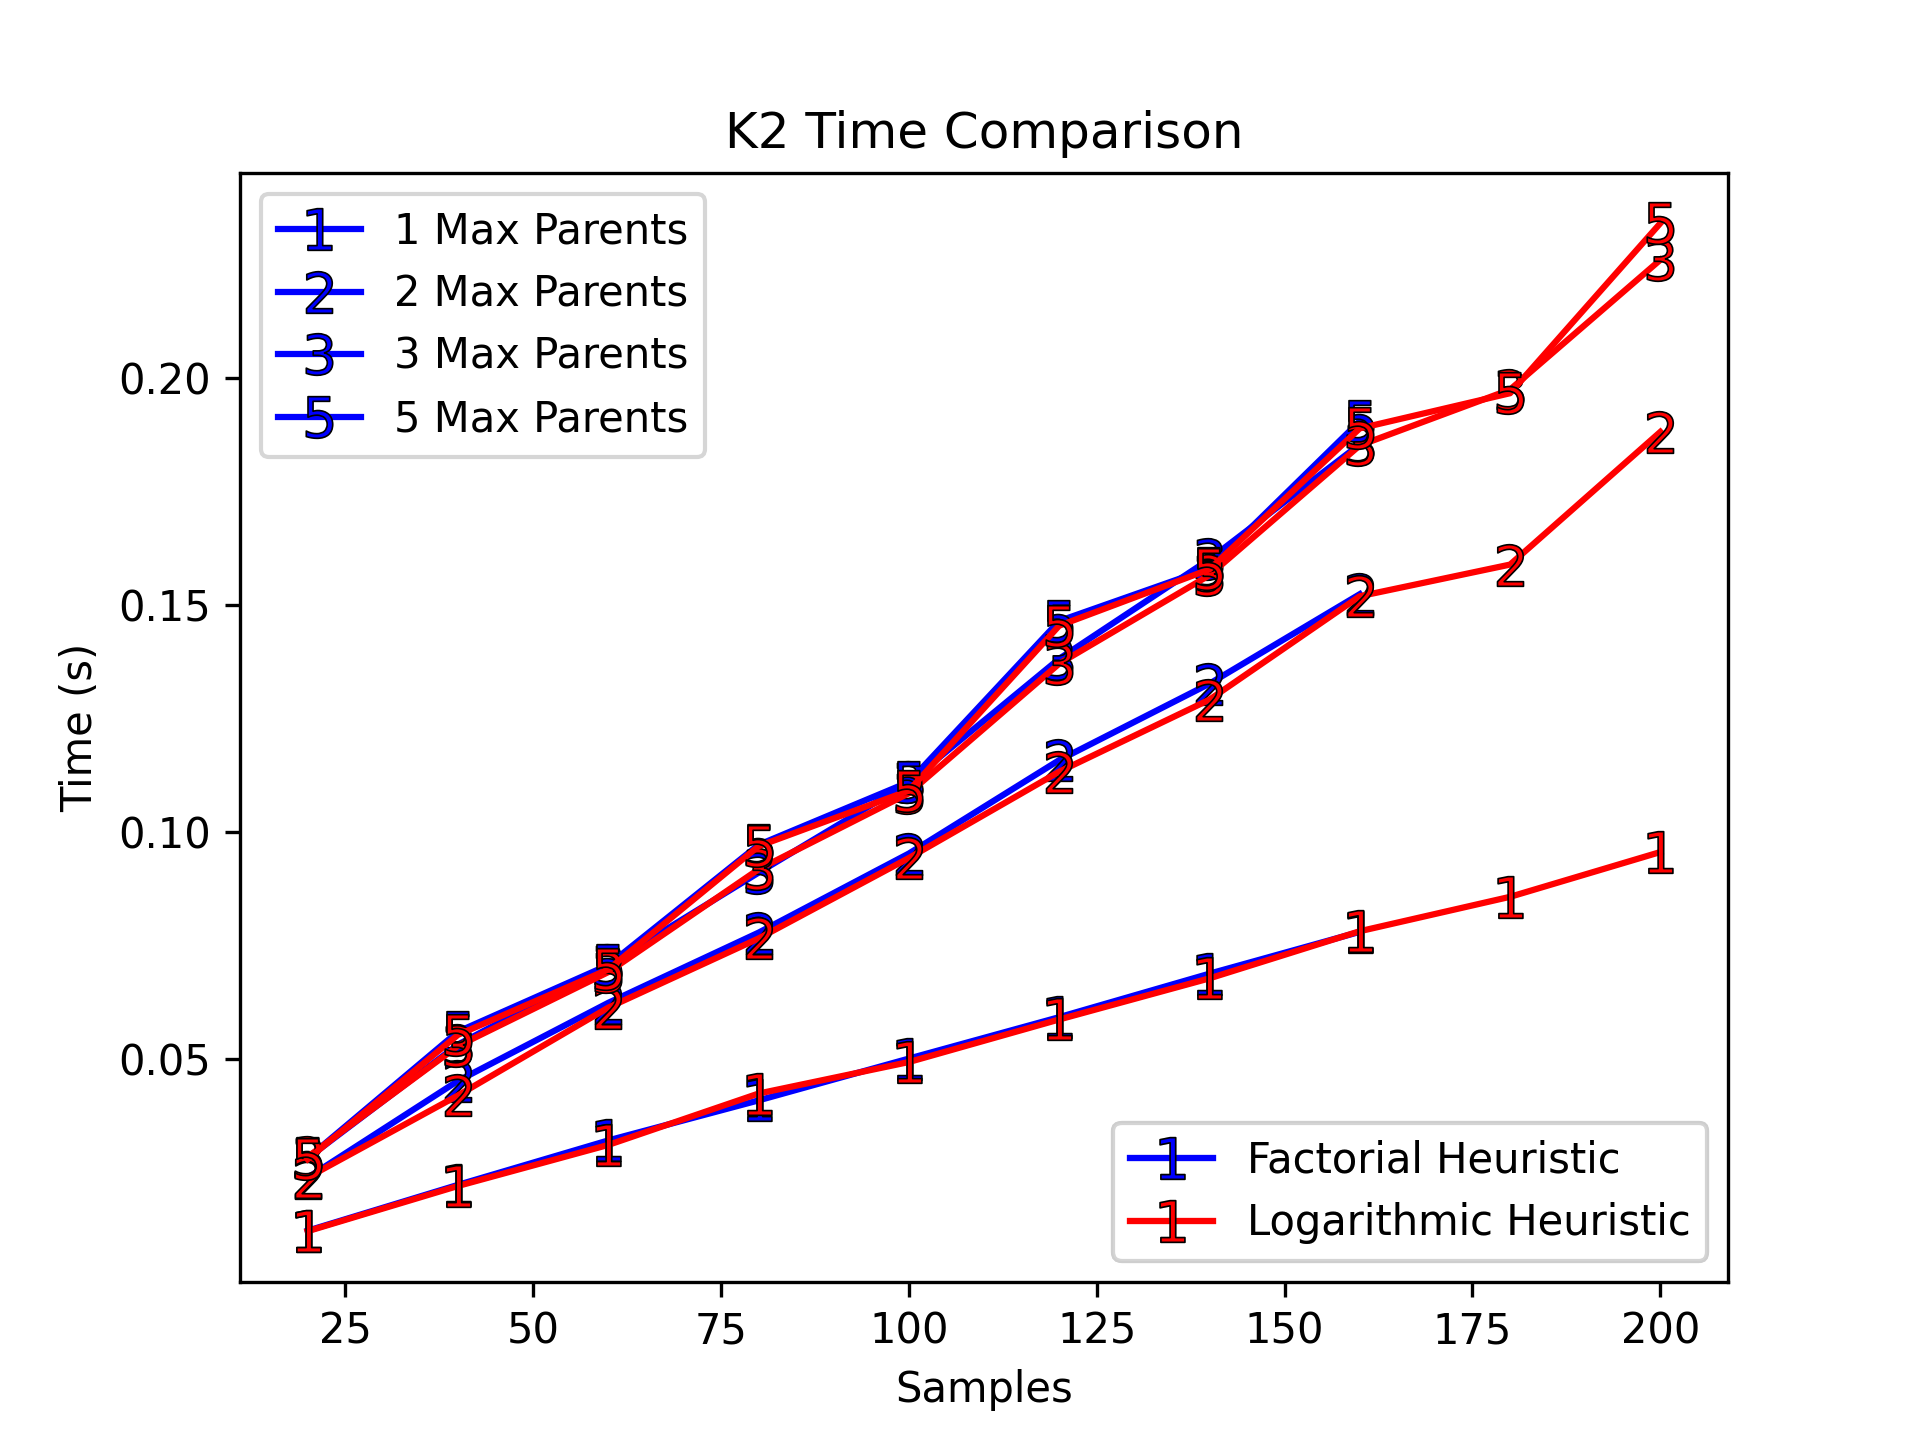
\includegraphics[width=0.75\textwidth]{k2_times.png}
    \caption{grafico che rappresenta i tempi di esecuzione di \textit{K2}}
    \label{fig:test1}
\end{figure}

I risultati sono rappresentati in figura \ref{fig:test1} e in linea con quanto riportato
nell'articolo\footnotemark[3]: i tempi di \textit{K2} risultano lineari rispetto al numero di
campioni, e si può notare che man mano che si aumenta il numero massimo di dipendenze condizionali
i tempi aumentano fino a arrivare a un \textit{plateau}: infatti con massimo uno o due dipendenze
condizionali per nodo notiamo differenze nei tempi, mentre per le curve con massimo tre e cinque
dipendenze non notiamo particolari differenze; questo è dovuto al fatto che la funzione euristica
blocca in anticipo l'estensione del numero dei padri osservando valori della funzione euristica
peggiori. Per quanto riguarda il tipo di funzione euristica applicata non si notano alcune
differenze sui tempi, ma è possibile osservare un'altro fenomeno: oltre 160 campioni l'algorimo con
l'euristica fattoriale fallisce nell'esecuzione per errori di \textit{overflow}, mentre applicando
l'euristica logaritmica non si hanno problemi di questo tipo; questo si spiega dal fatto che la
funzione euristica fattoriale genera punteggi molto bassi in modulo che devono essere moltiplicati
per fattoriali di numeri molto elevati.


\subsection{Secondo Test}

Sfruttando lo stesso script \textit{Python} del primo test, si analizzano le capacità
dell'algoritmo \textit{K2} nel ricondurre i campioni della distribuzione alla distribuzione
originale stessa. Per fare ciò si utilizza la misura di differenza tra i collider delle reti
bayesiane definita al punto 1.2, e si analizza la variazione di tale misura al variare del numero
di campioni, del numero massimo di dipendenze condizionali per ogni nodo e dell'euristica
utilizzata.

\subsubsection{Risultati}

\begin{figure}[h]
    \centering
    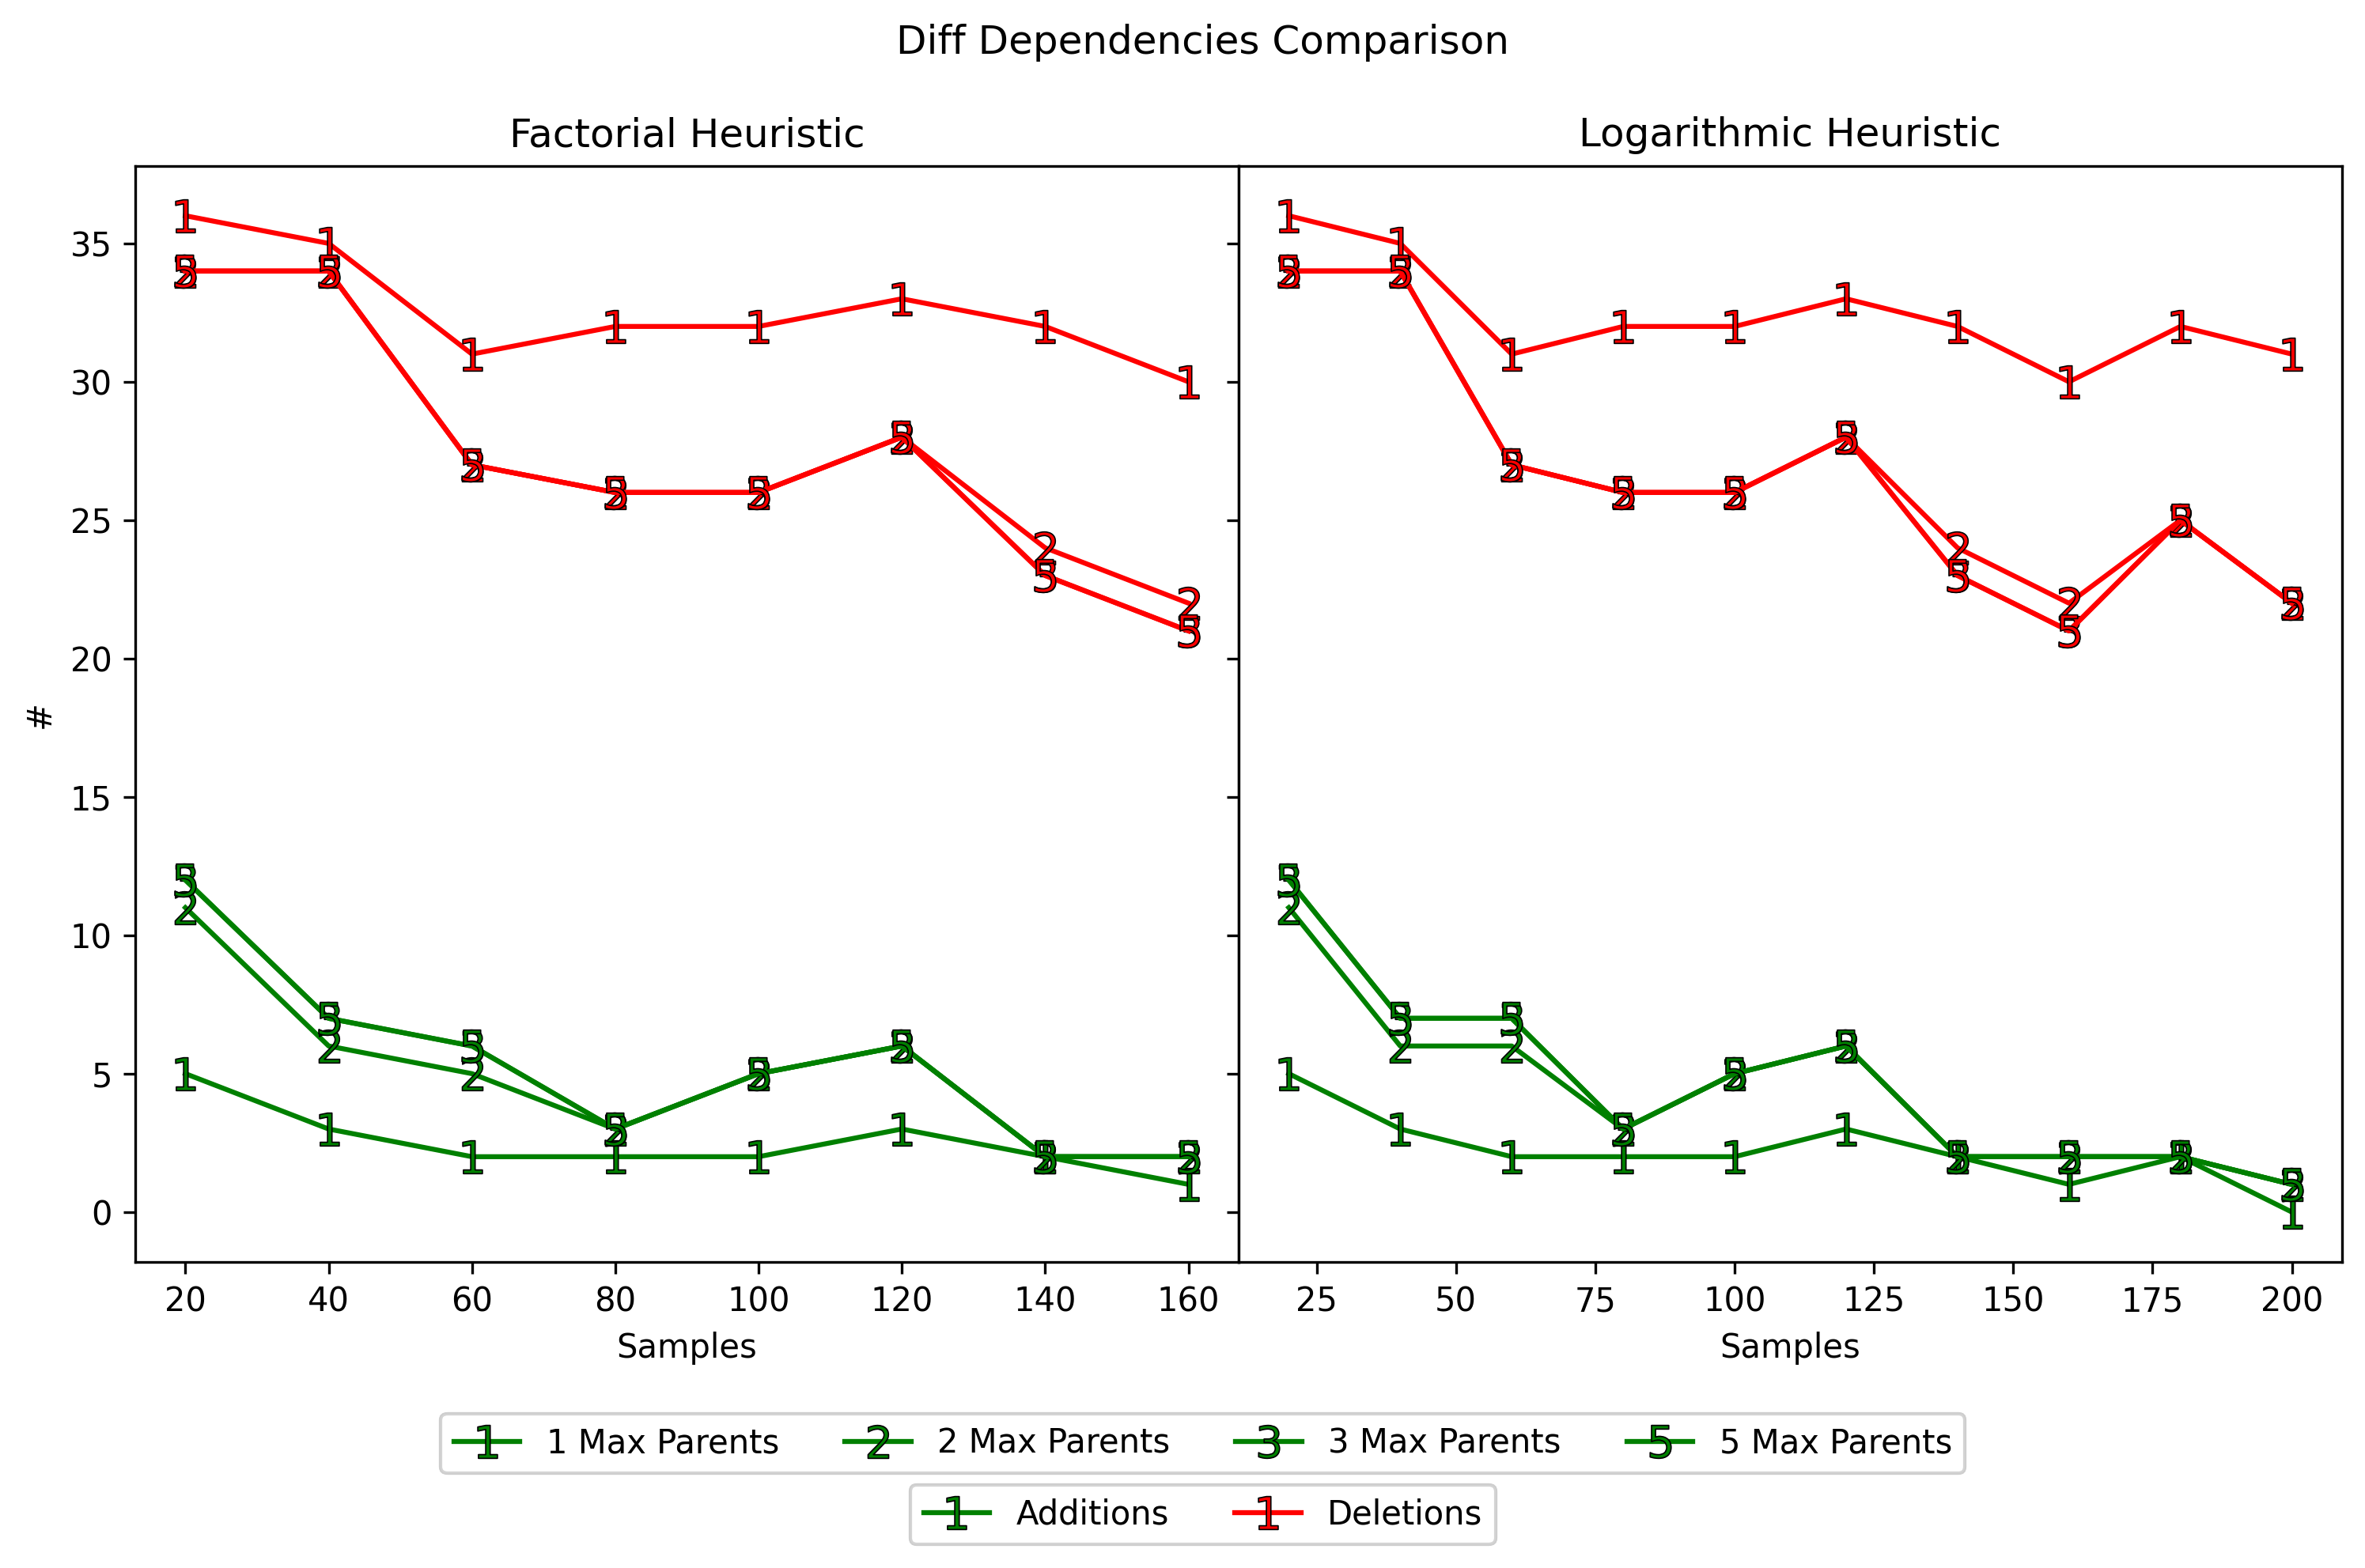
\includegraphics[width=0.9\textwidth]{diffs_deps.png}
    \caption{grafico che rappresenta il numero di collider in eccesso e difetto rispetto alla rete
        originale all'aumentare del numero dei campioni}
    \label{fig:test2}
\end{figure}

I risultati rappresentati in figura \ref{fig:test2} dimostrano che non c'è alcuna differenza
relativamente all'analisi tra l'utilizzo dell'euristica fattoriale e logaritmica, trascurando il
fatto che la variante logaritmica non fallisce dopo 160 campioni. In entrambi casi possiamo
osservare che aumentando il numero di campioni le discrepanze tra le reti diminuiscono. Analizzando
invece il comportamento al variare del numero massimo di dipendenze si nota che con tale limite
impostato a 1 si ha la possibilità di ottenere reti con meno collider aggiunti, a discapito di
quelle rimosse che risultano maggiori rispetto agli altri limiti; con limiti più alti (2, 3 e 5) si
hanno comportamenti simili che tendono a ridurre il più possibile il numero di collider in
eccesso/difetto. Notiamo comunque che l'algoritmo fatica molto più ad aggiungere eventuali collider
piuttosto che rimuoverne. In figura \ref{fig:test2:2} si possono osservare le reti generate.

\begin{figure}
    \centering
    \subfloat[\centering Con 20 campioni]{{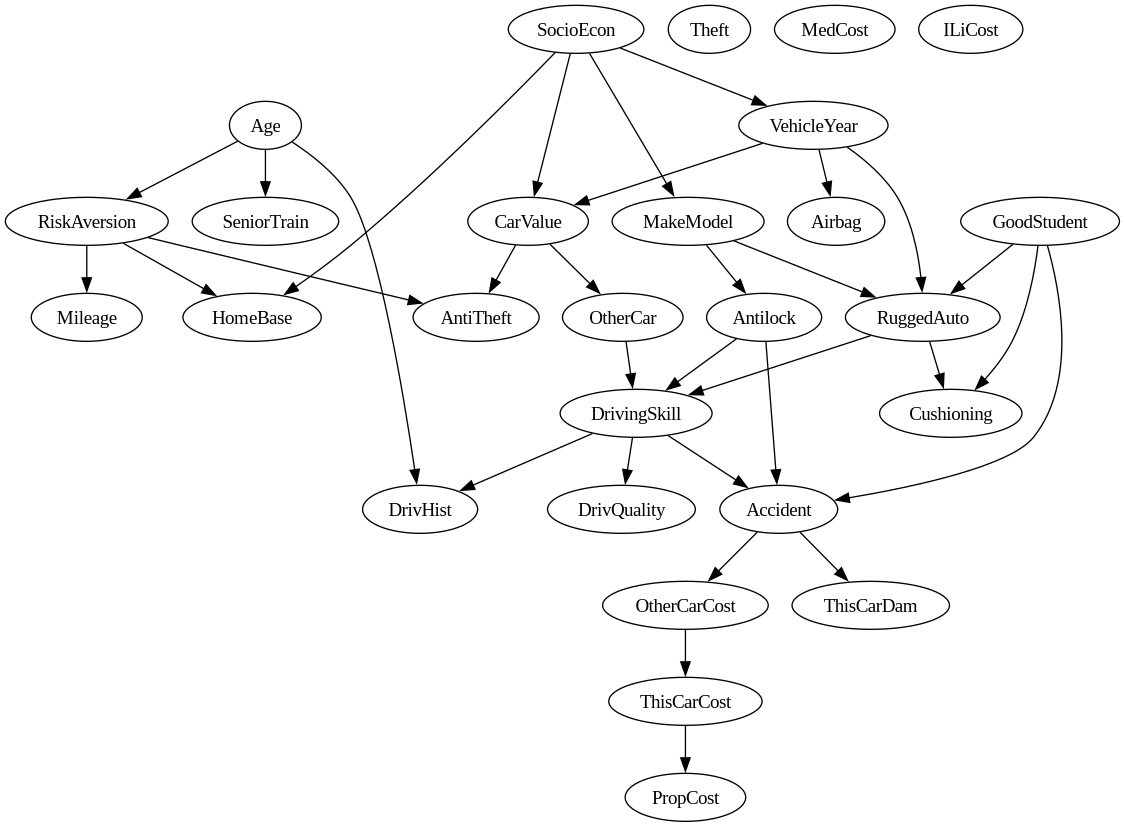
\includegraphics[width=8cm]{graph_20.png} }}
    \qquad
    \subfloat[\centering Con 200 campioni]{{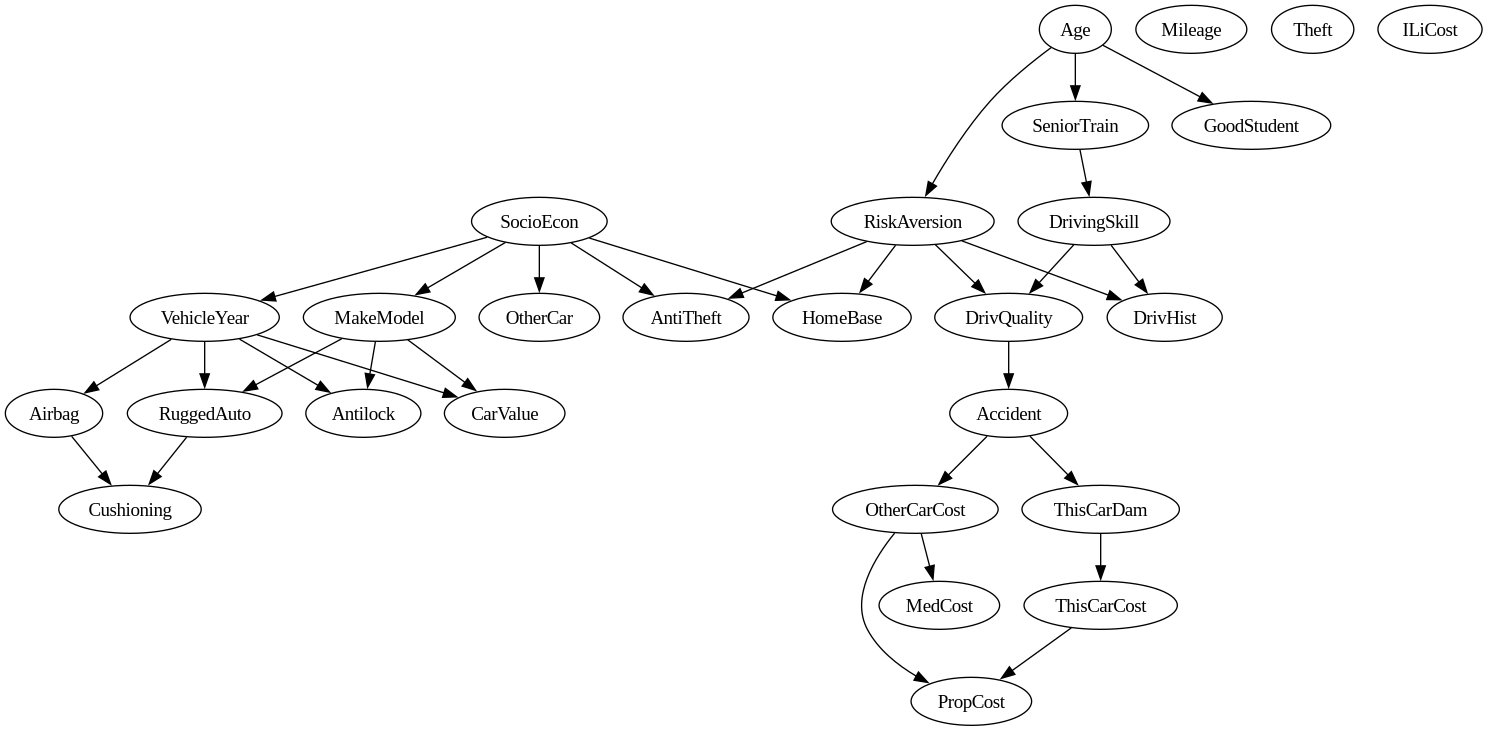
\includegraphics[width=8cm]{graph_200.png} }}
    \caption{Reti bayesiane generate con massimo 5 padri per nodo; i nodi con bordo rosso indicano i collider; è possibile confrontare questi
        grafi con quello originale disponibile all'indirizzo \url{https://www.bnlearn.com/bnrepository/insurance/insurance.svg}}
    \label{fig:test2:2}%
\end{figure}


\subsection{Terzo test}

Sulla base dei risultati ottenuti nei test precedenti, si esegue un'ultima analisi per verificare
quanti campioni siano necessari per ridurre al minimo la discrepanza tra le reti generate e quella
di partenza, misurando anche il tempo necessario. Per fare ciò si utilizza lo script
\texttt{min\_diff.py} che genera insiemi di campioni di cardinalità $1000 \cdot 2^x$ con $1 \le x
    \le 8$ sui quali viene eseguito l'algoritmo di apprendimento tramite l'euristica logaritmica (dato
che quella fattoriale fallisce dopo 160 campioni).

\subsubsection{Risultati}

\begin{figure}[h]
    \centering
    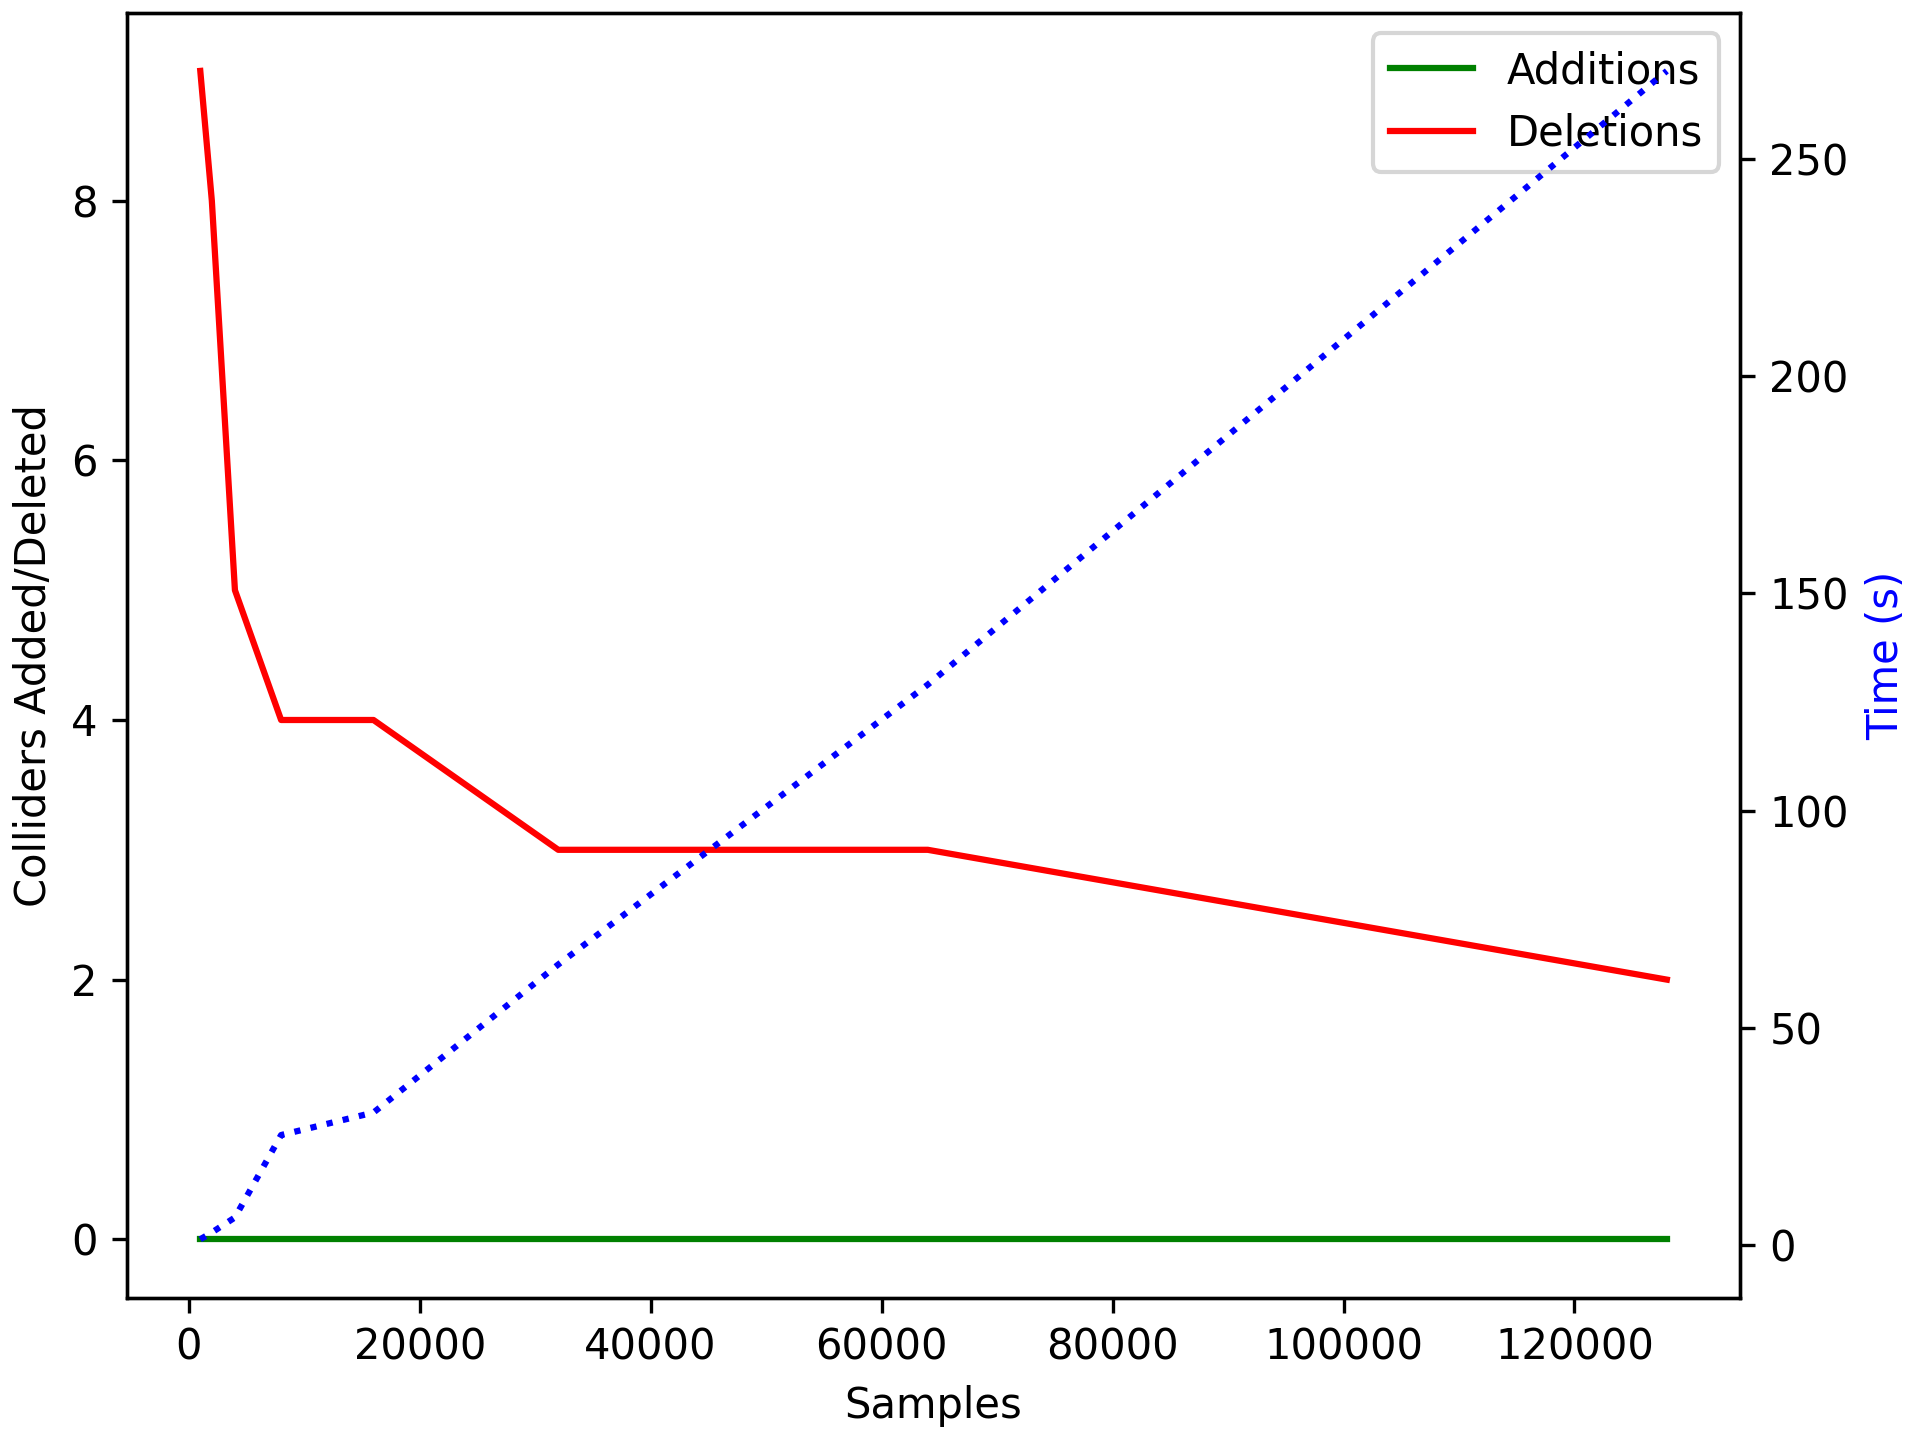
\includegraphics[width=0.6\textwidth]{min_diff.png}
    \caption{relazione tra il numero di collider errati e il numero di campioni; sull'ordinata destra è indicato il tempo di esecuzione}
    \label{fig:test3}
\end{figure}

Si può notare che nonostante un numero esponenziale di campioni, la rete generata non risulta
identica a quella di partenza da cui è stata generata la distribuzione, infatti il numero di
collider in eccesso raggiunge lo zero, ma il numero di collider in difetto diminuisce in maniera
molto lenta. Questo può indicare che l'algoritmo cerca di approssimare la rete ad una rete più
"\textit{libera}" che contiene meno dipendenze condizionali. Si è preferito fermarsi a 128000
campioni in quanto oltre tale soglia i tempi di esecuzione diventano superiori ai 5 minuti.

\section{Conclusioni}

Dobbiamo ribadire che tutti i test svolti assumono che l'ordine delle variabili preso in
considerazione dall'algoritmo sia ottimale, ovvero che ogni nodo sia figlio solamente di nodi
precedenti rispetto all'ordinamento; questo è un requisito molto forte che non è sempre verificato,
infatti in scenari di apprendimento di reti bayesiane spesso abbiamo a disposizione solamente un
insieme di campioni i.i.d.. A tal proposito l'articolo propone (in maniera generica) di sfruttare
un qualsiasi algoritmo di ricerca locale per individuare tra diversi ordinamenti casuali di
variabili il migliore eseguendo \textit{K2} su di esso e determinando un punteggio per la struttura
generata\footfullcite{LSEARCH:CH:1992}.

\end{document}